\documentclass[sigconf,review]{official-template/acmart}
% Official EDBT 2027 A4 geometry, copied verbatim from the downloaded template.
\geometry{twoside=true, head=13pt, a4paper, includeheadfoot, columnsep=2pc,
 top=57pt, bottom=73pt, inner=54pt, outer=54pt, marginparwidth=2pc,heightrounded}
\AtBeginMaketitle{\input{official-template/edbt-macros}}
\usepackage{graphicx,booktabs}
% Avoid font expansion failures in environments that only provide bitmap fonts.
\microtypesetup{expansion=false}
\title{[Vision Paper] From Papers to Scoped Theorems: Evidence-Grounded Knowledge Infrastructure for Database Theory}
\author{Liuye Hua}
\orcid{0009-0000-2122-0764}
\affiliation{%
  \institution{School of Computer Science and Technology}
  \institution{Innovation and Entrepreneurship Workshop}
  \institution{Xinjiang University}
  \city{Urumqi}
  \country{China}}
\email{hualiuye@stu.xju.edu.cn}

\author{Jiong Zheng}
\authornote{Corresponding author.}
\affiliation{%
  \institution{School of Computer Science and Technology}
  \institution{Innovation and Entrepreneurship Workshop}
  \institution{Xinjiang University}
  \city{Urumqi}
  \country{China}}
\email{zhengjiong@xju.edu.cn}
\renewcommand{\shortauthors}{Hua and Zheng}
\begin{document}
\begin{abstract}Database-theory results are routinely flattened into titles, citations, or one-sentence claims, losing the conditions that determine what was proved. We argue for a scope-preserving theorem atlas in which formal scope, source evidence, paper version, proof technique, and typed relations are first-class data. A bounded prototype---3,356 canonical paper families and a formally audited 20-paper/127-record batch---shows construction and auditing feasibility, not effectiveness or completeness. We identify the missing dimension across scholarly knowledge graphs, evidence models, mathematical knowledge systems, and formal libraries, and set a nine-part research agenda for extraction, verification, formal integration, relation inference, version evolution, open-problem status, benchmarks, governance, and human--AI collaboration.\end{abstract}
\keywords{database theory, scholarly knowledge graphs, theorem representation, provenance, research infrastructure}
\maketitle
\section{Introduction: Scope Loss} A theorem is not merely a sentence. In database theory its meaning may depend jointly on query fragment, fixed/input roles, structural restrictions, complexity regime, preprocessing, delay or access time, communication rounds, load, randomness, and conditional hypotheses. Dropping one axis can turn a valid theorem into a misleading claim. We argue for treating theorem scope and source evidence as first-class objects in scholarly infrastructure for database theory.
\section{Why Existing Infrastructure Is Insufficient} ORKG represents research contributions, comparisons, provenance, and versions; micropublications and nanopublications represent claims and evidence; PAV represents provenance and versioning; OntoMath, OMDoc/MMT, and Mizar represent mathematical objects and formal dependencies; S2ORC and SciFact provide document and evidence substrates. These are foundations, not absences. The missing dimension is a prescribed, source-bound database-theory scope contract with explicit unknowns and fail-closed promotion.
\begin{figure}[t]\centering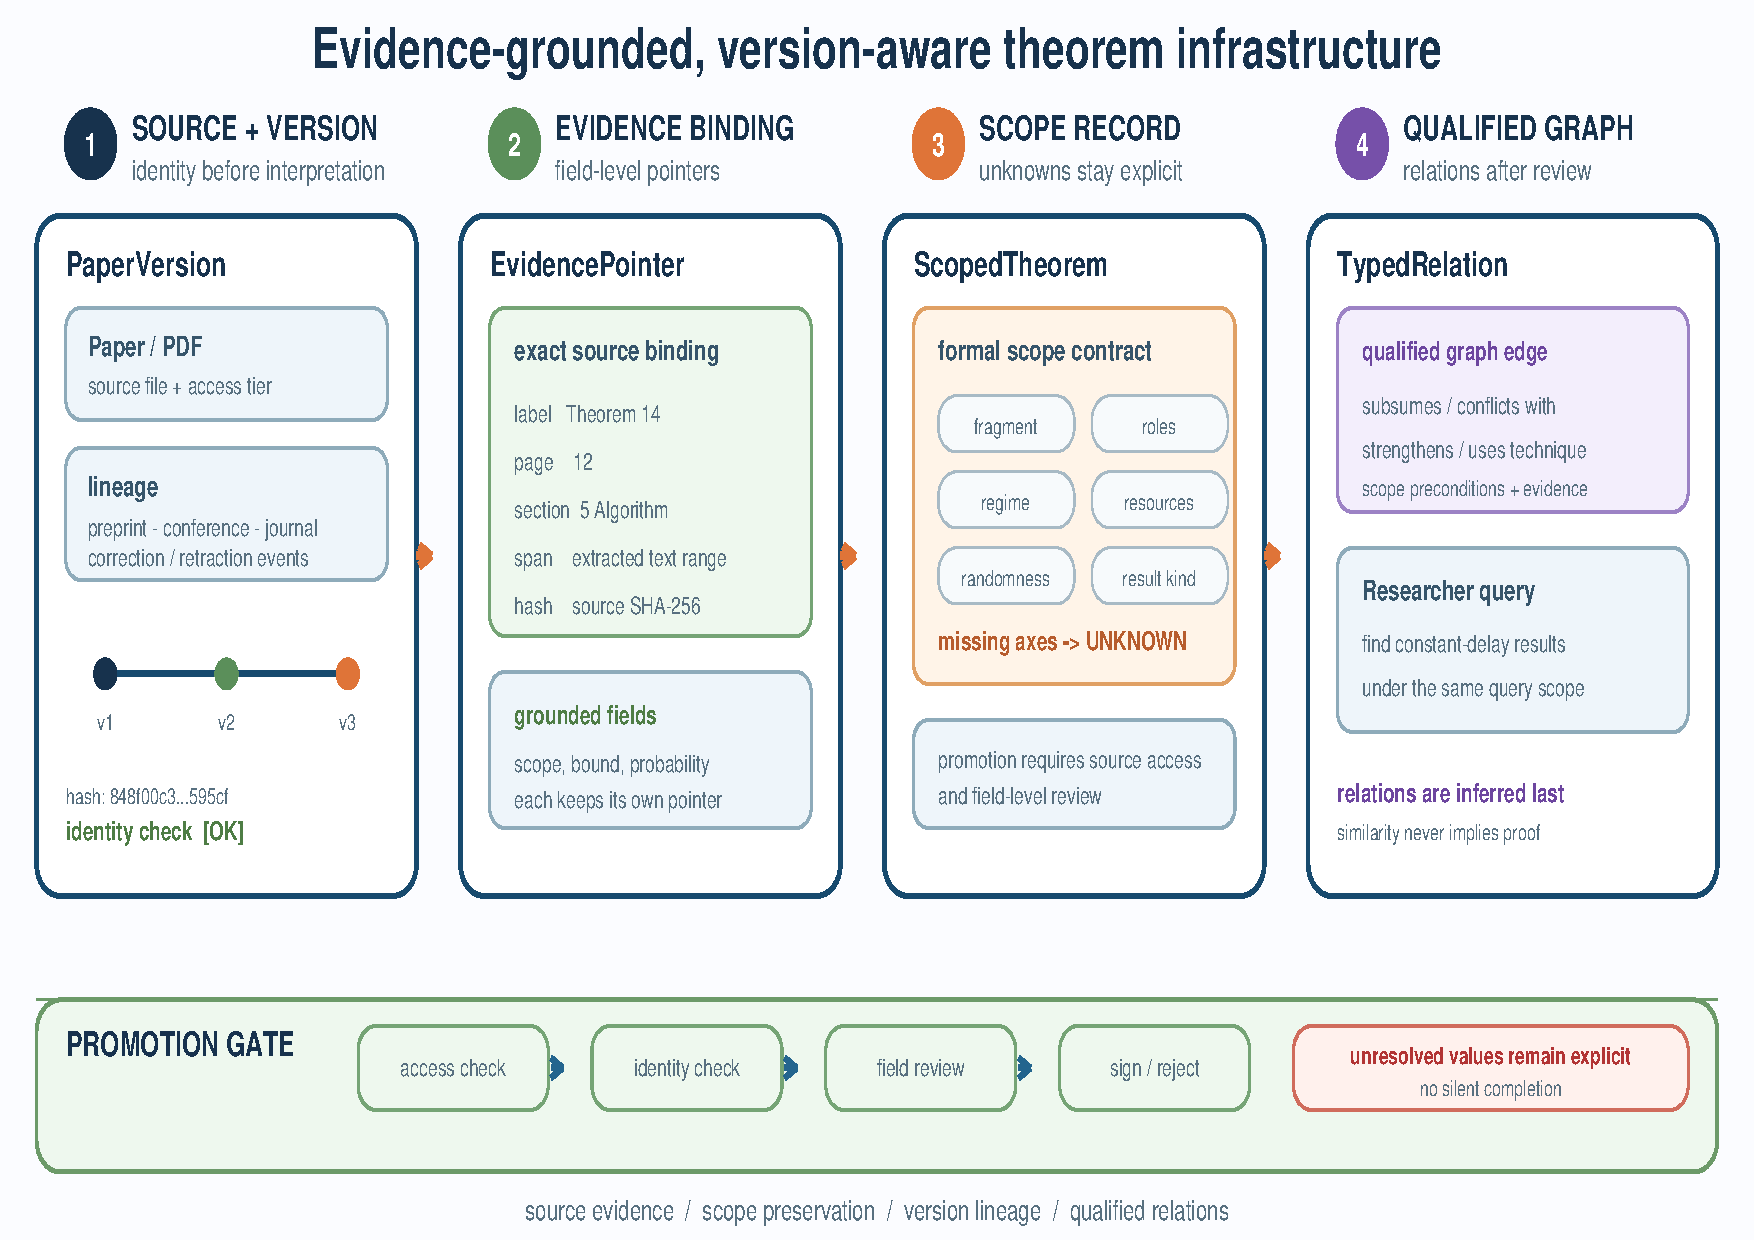
\includegraphics[width=\columnwidth]{figures/architecture.pdf}\caption{Evidence and version identity constrain promotion into scoped theorem records before typed graph relations are inferred.}\end{figure}
\section{A Scope-Preserving Theorem Atlas} A \texttt{ScopedTheorem} records the formal problem, fragment, assumptions, parameter roles, complexity regime, resource bounds, randomness, and result kind. An \texttt{EvidencePointer} binds fields to label, page, section, source hash, and extraction span. A \texttt{PaperVersion} distinguishes conference, journal, preprint, correction, and retraction lineage. \texttt{ProofTechnique} and qualified \texttt{TypedRelation} objects support navigation without pretending that similarity is implication. Promotion requires source access, identity validation, field-level review, and unresolved values remaining explicit.
\begin{figure}[t]\centering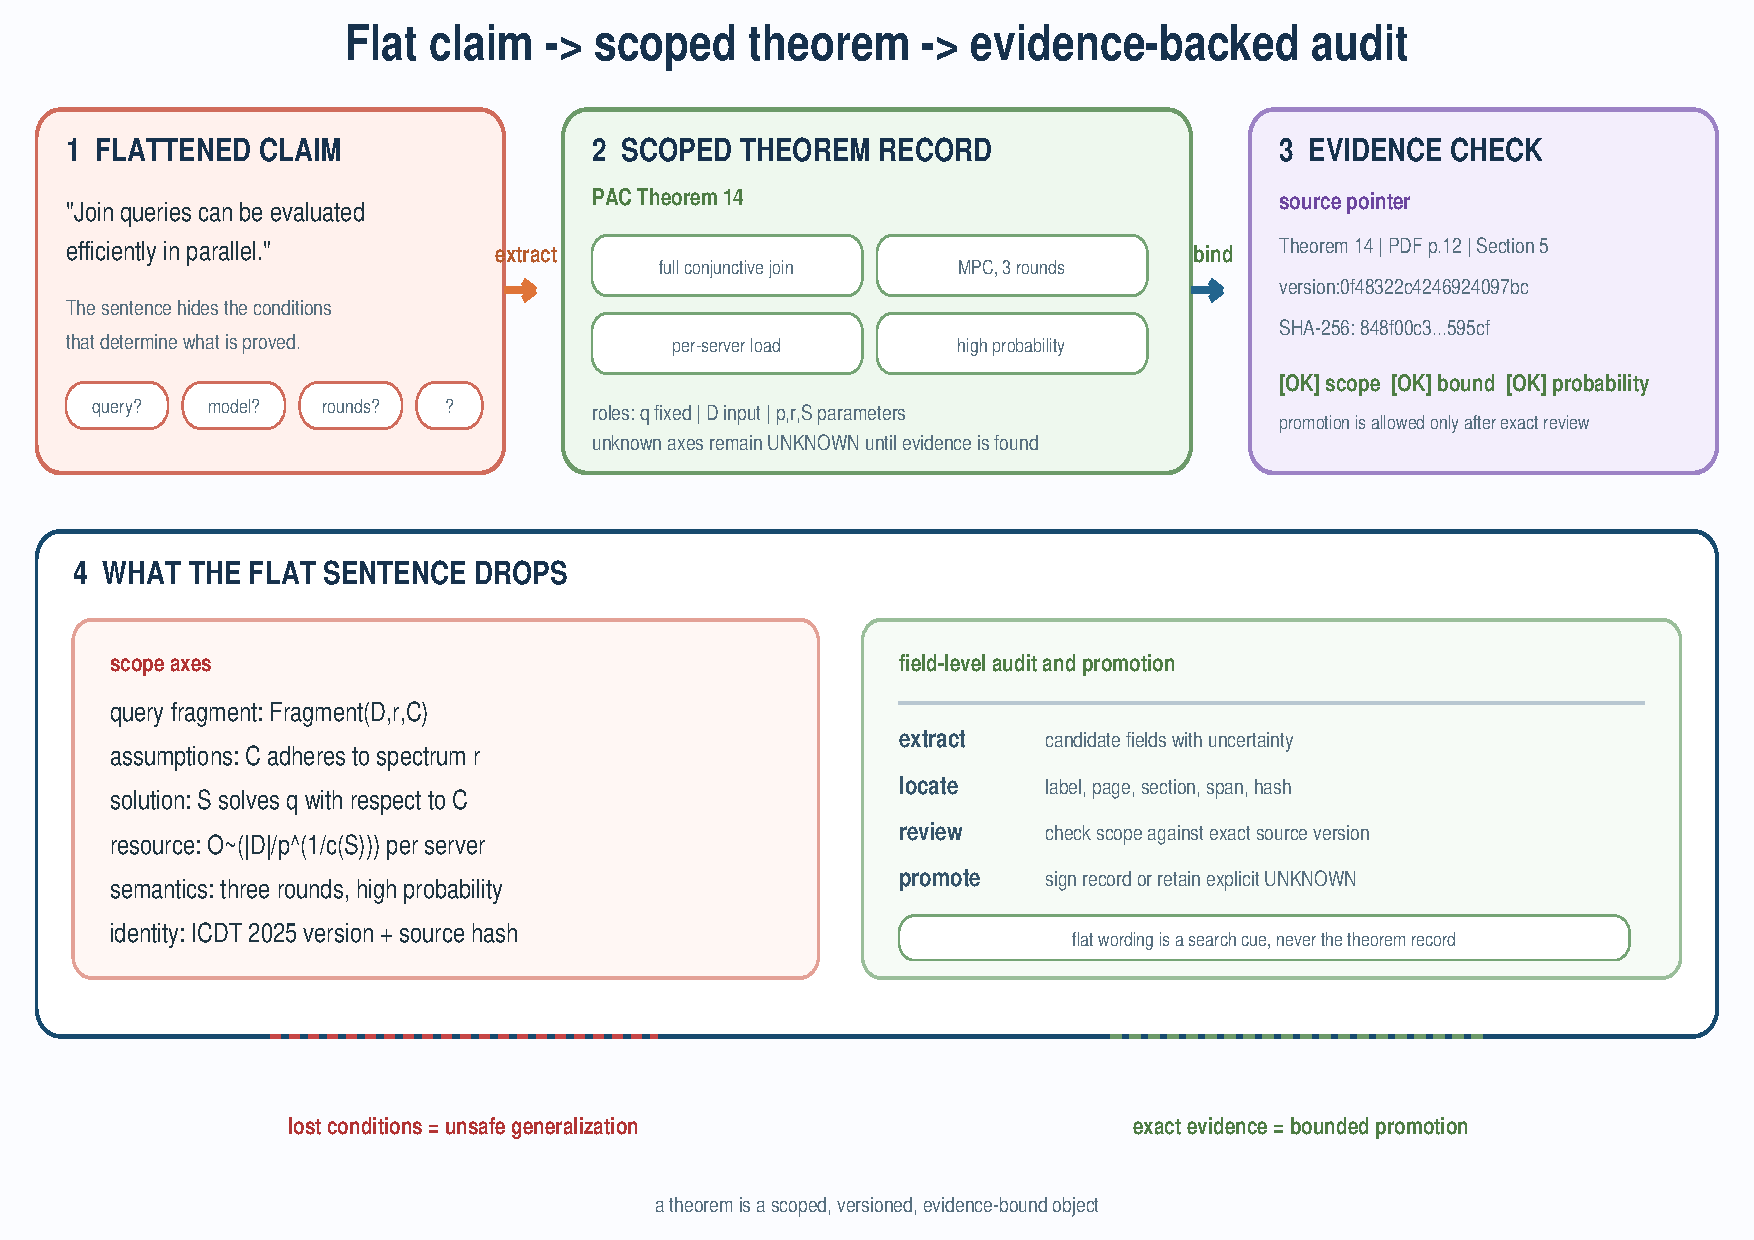
\includegraphics[width=\columnwidth]{figures/running_example.pdf}\caption{A flattened claim drops the conditions that delimit PAC Theorem 14.}\end{figure}
\section{Feasibility Prototype} The frozen workflow contains 3,737 provider observations consolidated into 3,356 canonical families; 309 were marked relevant by deterministic screening. The read-depth ledger records 125 FULL\_SCAN and 80 DEEP\_READ papers. The admissible theorem batch covers 20 papers and 127 theorem/proposition records, all with source locations and 20 distinct version IDs. Every number is recomputable from hashed artifacts. These counts establish bounded feasibility and auditability only.
\section{Research Agenda} \textbf{A Extraction:} generate field candidates with calibrated uncertainty; evaluate field precision/recall and abstention against expert records. \textbf{B Scope verification:} detect missing or conflicting axes through document context and cross-version constraints; score axis-level agreement. \textbf{C Formal integration:} link informal records to proof-assistant declarations while retaining evidence; evaluate alignment coverage and soundness. \textbf{D Relation inference:} propose qualified subsumption, strengthening, incompatibility, and technique edges; evaluate expert acceptance and logical counterexamples. \textbf{E Evolution:} model theorem identity across preprint, conference, journal, correction, and retraction; evaluate lineage reconstruction. \textbf{F Open problems:} store evidence-qualified status events rather than timeless labels; evaluate freshness and false-closure rates. \textbf{G Benchmarks:} create stratified tasks for extraction, evidence retrieval, scope comparison, and research navigation; report calibration and cost, not only accuracy. \textbf{H Governance:} design roles, disputes, credit, vocabulary evolution, and sustainable curation; evaluate latency and agreement. \textbf{I Human--AI collaboration:} optimize candidate generation, explanation, and fail-closed review; evaluate error escape, workload, and trust.
\section{Risks, Governance, and Limitations} Risks include authoritative-looking errors, coverage bias, terminology drift, source disappearance, credit distortion, and stale open-problem status. Mitigations are explicit provenance, immutable source/version identity, uncertainty, competing annotations, signed promotion, appeal paths, and periodic audit. The prototype does not measure extraction accuracy, usefulness, adoption, or completeness and does not replace formal proof.
\section{Conclusion} A scope-preserving theorem atlas is a database research agenda: representation, integrity constraints, provenance, entity resolution, uncertain extraction, version evolution, querying, benchmarks, and governance meet in one demanding scholarly domain.
\section*{Artifacts} The package includes code, schemas, derived metadata, audited structured records, scripts, tests, figures, and documentation; it excludes copyrighted source PDFs and unreviewed theorem batches. Rebuild instructions, hashes, definitions, and AI-use ledger are included. The public bounded release is available at \url{https://github.com/hly99999/edbt2027-vision-atlas/tree/v0.1.0}; the tag identifies the immutable release, while the exact commit is recorded in the release metadata.
\balance
\bibliographystyle{official-template/ACM-Reference-Format}\bibliography{references}\end{document}
